\documentclass[a4paper, 14pt]{extarticle}
\usepackage[dvipsnames]{xcolor}
\usepackage[top=70pt,bottom=70pt,left=48pt,right=46pt]{geometry}
\definecolor{header}{RGB}{92,184,92}
\definecolor{defenition}{RGB}{217,83,79}
\definecolor{main_title}{RGB}{66,139,202}
\definecolor{sub_header}{RGB}{91,192,222}
\usepackage[english, russian]{babel}
\usepackage[utf8]{inputenc}
\usepackage{amsmath}
\usepackage{listings}
\usepackage{graphicx}
\usepackage{amsmath}
\title{\textcolor{main_title}{Генераторы синусоидальных колебаний с кварцевой стабилизацией частоты}}
\author{Шмаков Владимир Евгеньевич - ФФКЭ гр. Б04-105}






\begin{document}
\maketitle



\section*{\textcolor{header}{Резонасный усилитель}}

\subsection*{\textcolor{sub_header}{Нахождение добротности резонансного усилителя}}


Снимем АЧХ резонасного усилителя и найдём его добротность(смотрите рисунок $\ref{fig:afr}$).
\begin{figure}[htbp]
    \centering
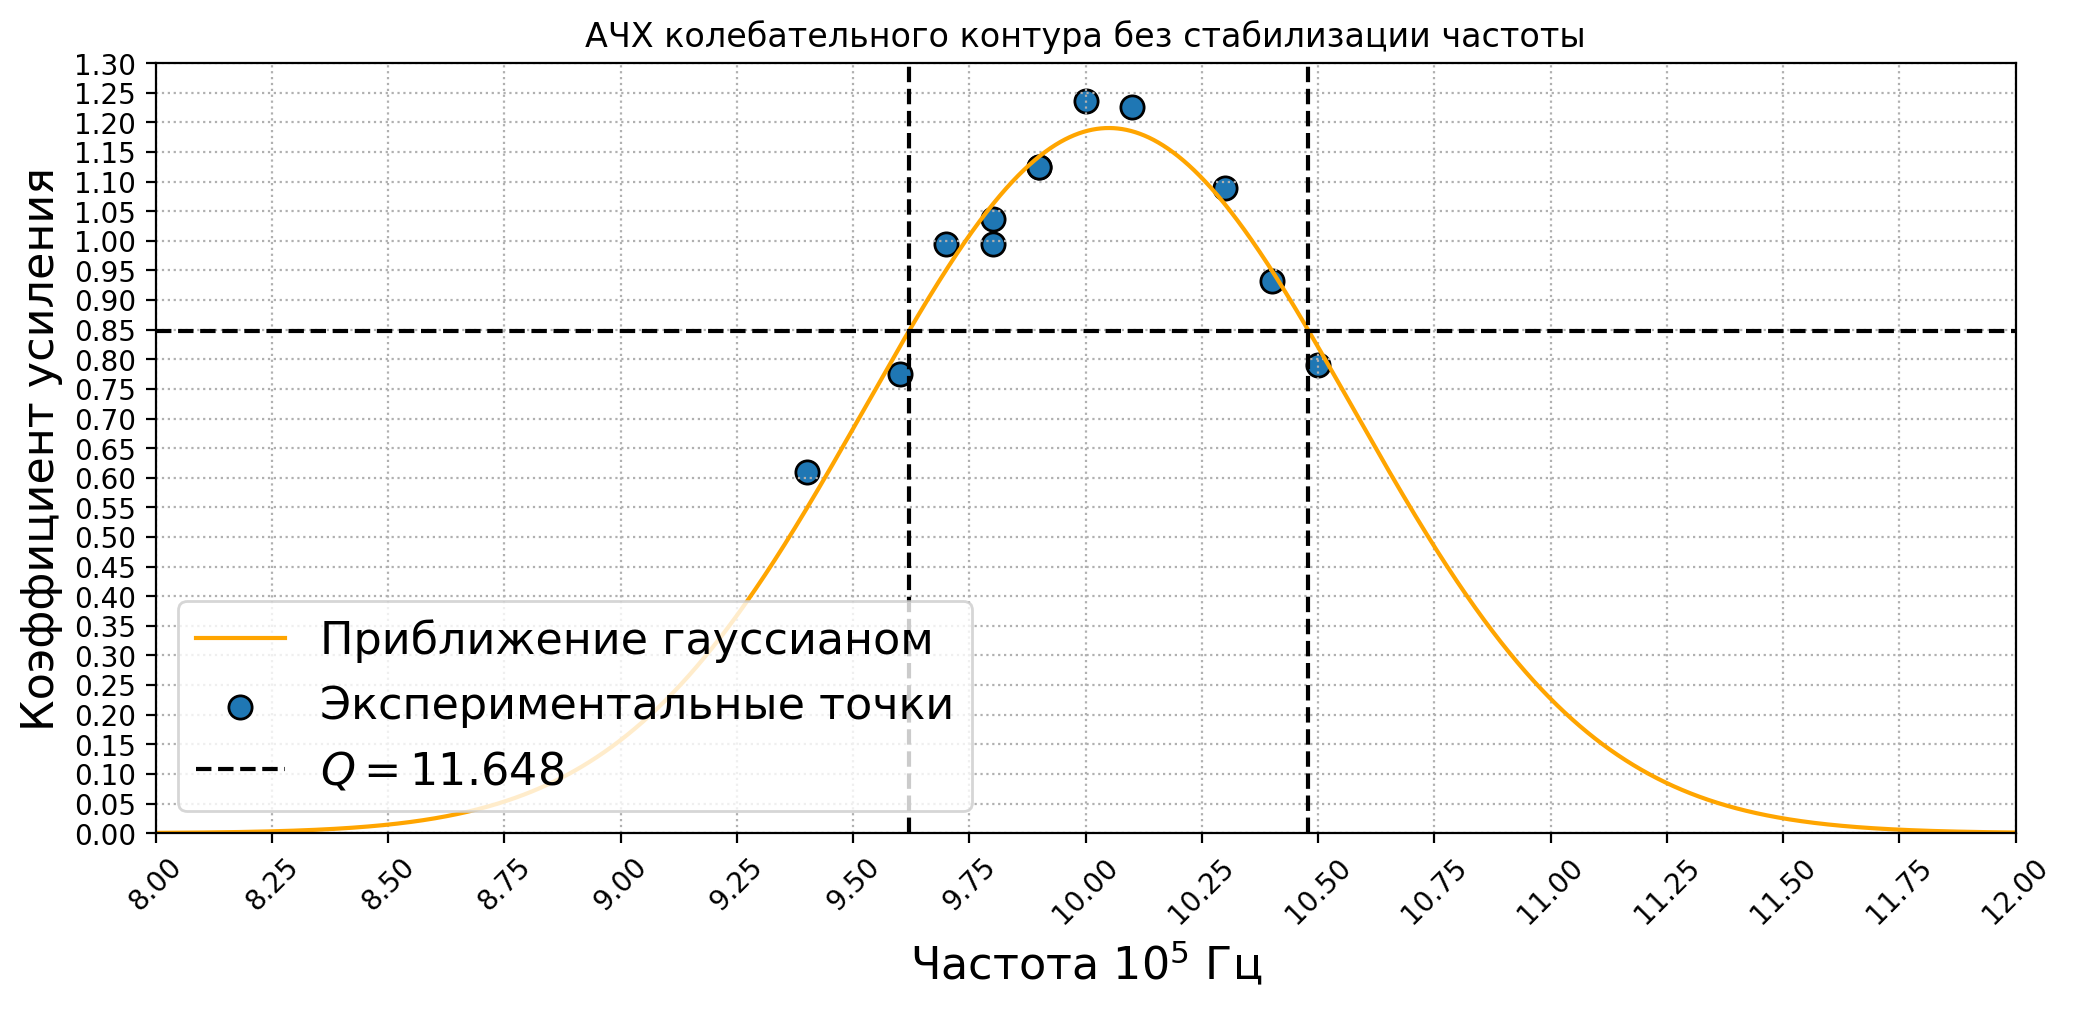
\includegraphics[width = 1 \textwidth]{afr.png}
    \caption{АЧХ резонасного усилителя}
    \label{fig:afr}
\end{figure}

\subsection*{\textcolor{sub_header}{Генерация синусоидальных колебаний посредством добавления обратной связи}}

Соединим выход схемы со входом. Таким образом, узкополосный резонатор <<превратится>> в генератор синусоидольного 
сигнала. 

\begin{figure}[htbp]
    \centering
    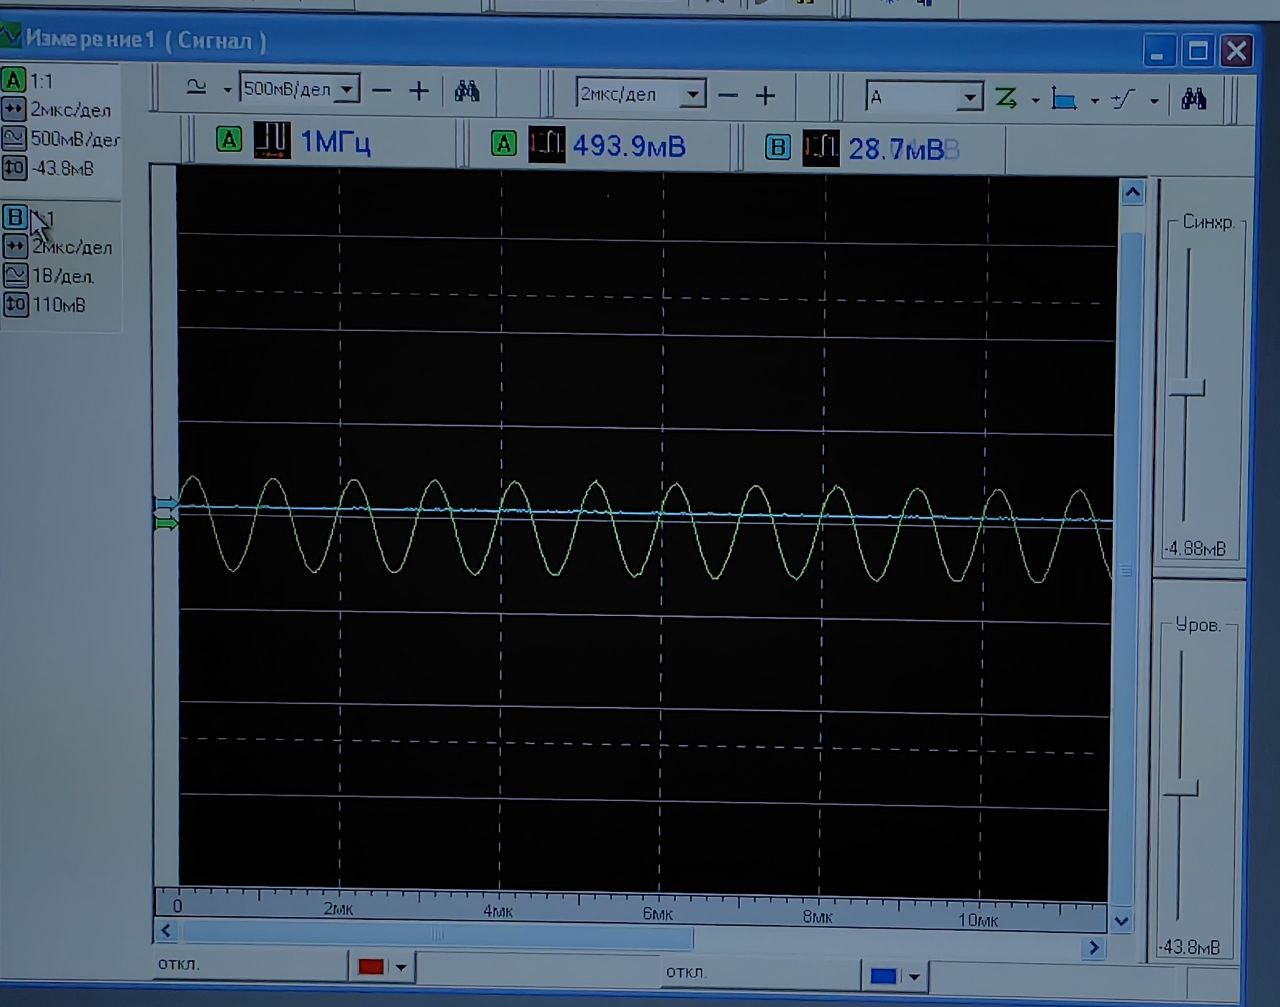
\includegraphics[width = 1\textwidth]{osc.jpg}
    \caption{Выходной сигнал генератора}
    \label{fig:osc}
\end{figure}

\section*{\textcolor{header}{Стабилизация частоты}}

\subsection*{\textcolor{sub_header}{Нахождение добротности кварцевого резонатора}}

Добавим в секцию $LC$ контура дополнительную ёмкость $C = 10 \text{пФ}$. 
При наличии в цепи кварцевого резонатора, 
частота меняется слабо: $\Delta f_{q} = 7 \text{ Гц}$. 
Если стабилизация частоты отсутствует, то частота меняетс на $\Delta f \sim 18 \text{ кГц}$. 

Полученные данные позволяют найти добротность кварцевого резонатора:
\begin{equation}
    Q_{\text{к}} = \frac{\Delta f Q}{\Delta f_{q}} \sim 3 \cdot 10^{4}
\end{equation}

Получили что добротность кварцевого резонатора достаточно высока, как и добротность любой
акустической системы. Для сравнения, добротность струны $\sim 10^3$.

\subsection*{\textcolor{sub_header}{Исследование стабильности частоты кварцевого генератора}}

Построим график зависимости частоты генерации в зависимости от напряжения питания.

\begin{figure}[htbp]
    \centering
    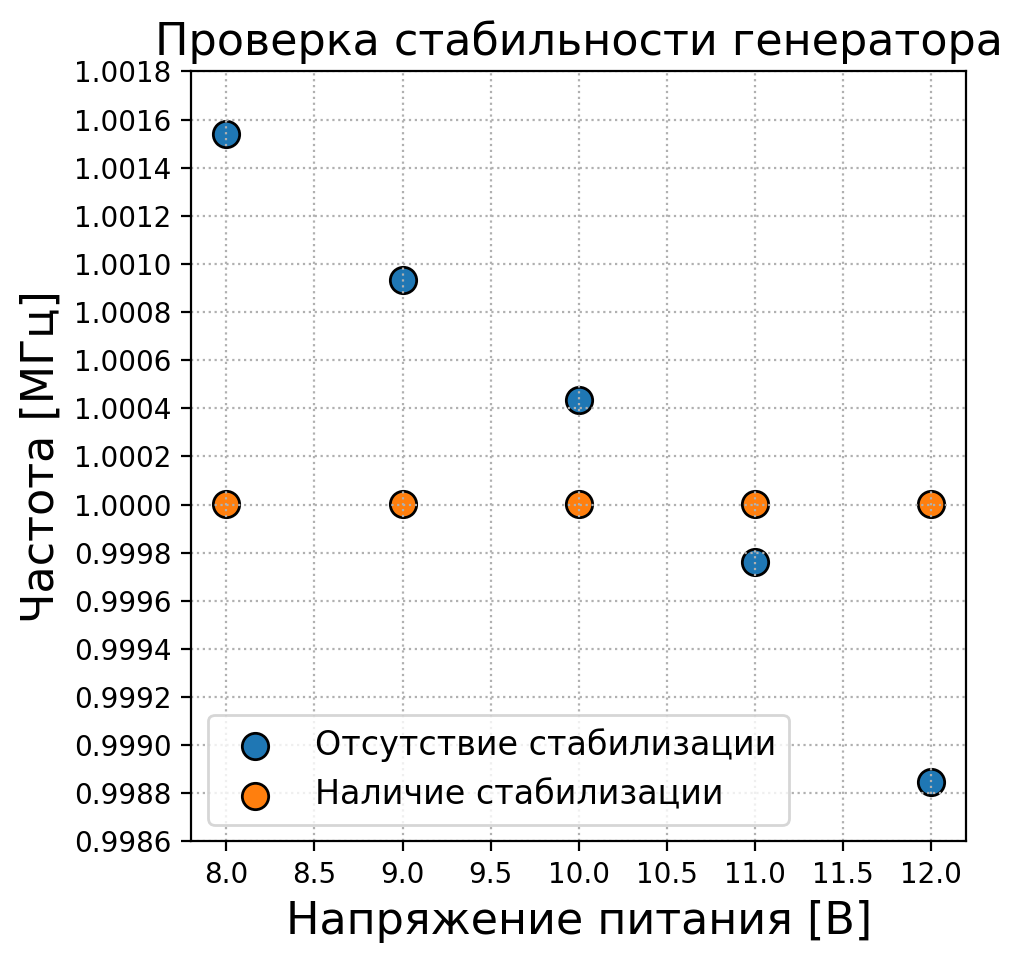
\includegraphics[width = 0.5 \textwidth]{stabil.png}
    \caption{Исследование зависимости частоты генерации от напряжения}
    \label{fig:stabil}
\end{figure}

Как видно на рисунке $\ref{fig:stabil}$ в отсутствие кварцевого резонатора, 
частота линейно падает с ростом напряжения питания. В схеме со стабилизацией,
частота меняется максимум на $10 \text{ Гц}$.  

\subsection*{\textcolor{sub_header}{Определение параметров кварцевого резонатора}}

Последовательно с кварцевым резонатором подключим конденсатор ёмкостью $C_{s} = 120 \text{ пФ}$.
При этом частота генерации изменится на $\Delta f_{k} = 0.007 \text{ МГц}$. 

\begin{equation*}
C_{k} = \frac{2 \cdot C_{s} \Delta f_{k}}{f_{k}} = 1.68 \text{ пФ}
\ \
L_{k} = \frac{1}{4 \pi^{2} f_{k}^{2} C_{k}} = 0.015 \text{ Гн}
\ \ 
r_{k} = \frac{2 \pi f_{k} L_{k}}{Q_{k}} = 3.16 \text{ Ом}
\end{equation*}


\end{document}
